Realizzare simulazioni di processi LMD senza avvalersi di software CFD sarebbe pressoché impossibile.
Al momento il settore dei software per CFD è ricco di strumenti e applicazioni, che attraverso processi semplificati e interfacce intuitive,
rendono molto più veloce e semplice tutto ciò che concerne il ciclo di progettazione di soluzioni che necessitano
analisi e test di flussi, deformazioni e molto altro.
Il problema principale che spesso è causa dell'inutilizzo di questi programmi è il costo di utilizzo in termini economici,
non è raro infatti imbattersi in licenze che superano anche i 50000 Euro/Anno per postazione.
Come abbiamo visto nel capitolo precedente esistono anche soluzioni open-source, molto popolari in ambito accademico, che però
richiedono conoscenze informatiche, oltre che matematiche e fisiche, avanzate per essere utilizzate correttamente. Avere a disposizione
il codice sorgente di uno strumento capace di risolvere PDE (\ref{PDE}) con FEM (\ref*{fem}) o FVM è un grande vantaggio, dà la possibilità di
comprendere meglio il funzionamento di simulazioni complesse e modificarlo a proprio piacimento.
In questo capitolo analizzeremo ciò che è stato prodotto da un punto di vista software, per soddisfare gli obiettivi prefissati.
In particolare discuteremo le scelte architetturali e i pattern software utilizzati, motiveremo le strutture dati e le librerie impiegate.

Lo sviluppo del simulatore ha subito diversi cambiamenti radicali durante lo svolgimento di questo percorso. Per ovviare alle difficoltà implementative
che questi cambiamenti ponevano si è subito cercato di compartimentalizzare ogni macro modulo di funzionalità per rendere più facile, veloce e collaborativo lo sviluppo.
Ogni modulo è orchestrato da un punto di ingresso (o \texttt{main}) che inizializza e coordina gli stessi al fine di produrre in output dei risultati.
Solitamente per simulare un evento fisico che si svolge in un intervallo di tempo continuo lo si discretizza introducendo il concetto di time-step. Il time-step
è ciò che determina la risoluzione temporale della simulazione, ovvero il lasso di tempo che passa tra un intervallo e il successivo.
Per esempio in un lasso di tempo di \(10\) secondi con un \texttt{dt} (delta temporale) di \(0.1s\) secondi otteniamo:
\[
    \frac{10s}{0.1s}=100 \text{ time-step}
\]
I time-step vengono utilizzati all'interno della simulazione per determinare quante volte viene eseguito il passo risolutivo di ogni modulo.

Di seguito è mostrato un diagramma dei moduli e la loro interazione:
\begin{figure}[H]
    \centering
    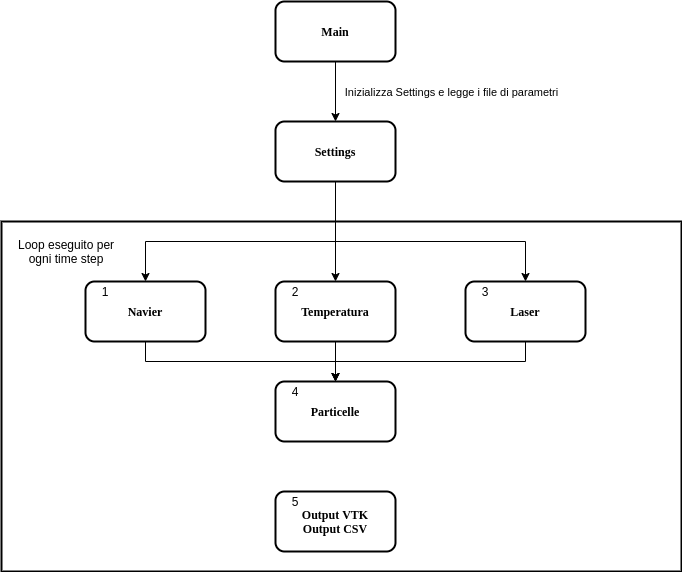
\includegraphics[width=\linewidth]{diagrammi/diagrammiModuli.png}
    \caption{Interazione fra moduli.}
\end{figure}
Personalmente all'interno del progetto ho partecipato più attivamente allo sviluppo del modulo Particellare (\ref*{5:particelle}), ma di seguito è riportata
una breve descrizione anche degli altri moduli. I moduli sono ordinati su base temporale, quindi dal primo utilizzato all'ultimo, viene inoltre fornito un diagramma di flusso per ognuno.

    \section{Gestione Input e impostazioni}\label{input}\label{settings}
    Per rendere il software adatto a diverse simulazioni in maniera intuitiva e veloce, è stato creato un modulo responsabile della gestione dei parametri iniziali di simulazione.
    Il modulo si avvale dell'interfaccia esposta dalla libreria deal.II (\ref{dealii}) \newline\texttt{deal.II\//base\//parameter\_handler.h}\label{parameterhandler}, che facilita la gestione di parametri e il
    relativo parsing da file (\texttt{parameter\_file.prm}).
    \begin{figure}[H]
        \centering
        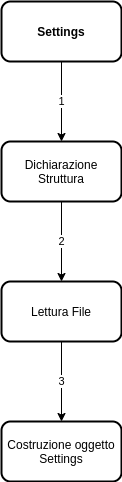
\includegraphics[width=0.3\textwidth]{diagrammi/diagrammiInput.png}
        \caption{Flusso di gestione input.}
    \end{figure}

        \subsection{Struttura file di input}
        Il file di parametri ha una struttura composta di diverse \texttt{section}, caratterizzate da un nome, e molteplici variabili che possono rappresentare sia numeri che stringhe.
        Le section possono anche essere annidate una dentro l'altra per avere a disposizione un ulteriore livello di organizzazione dei parametri.
        \begin{verbatim}
section Simulation parameters
    set simulation_time         = 0.2
    set time_step               = 0.1
    set theta                   = 1.0
    set mesh_file               = ../mesh/mesh.dealii
    set refinement_mesh_degree  = 1
end
        \end{verbatim}
        Analizzando la sottosezione del file di parametri si può notare come non vengono utilizzati nessun tipo di identificatore per distinguere i vari tipi di dato (numeri interi, decimali o stringhe), bensì
        tratta tutto ciò che viene posto dopo il segno di uguaglianza come semplici caratteri. Sarà infatti compito di \ref*{parameterhandler} distinguere i vari tipi in base alle istruzioni di dichiarazione
        in fase di parsing, istruzioni che vedremo nel dettaglio in \ref{implementazione_prm}.
        Il file può contenere un numero arbitrario di sottosezioni, è buona pratica però organizzare le sottosezioni in maniera analoga a quella del resto del progetto; ovvero compartimentalizzando
        le impostazioni rispettivamente alle proprie aree di interesse. Di seguito è rappresentata la struttura finale del file utilizzato per raggiungere i risultati di \ref{cap:capitoli/capitolo6/capitolo6}.

        \begin{verbatim}
section Simulation parameters
    set simulation_time         = 0.1
    set time_step               = 0.0002
    set theta                   = 1.0
    set mesh_file               = ../mesh/mesh.unv
    set refinement_mesh_degree  = 0
end

section FEM parameters
    set fe_degree               = 1
end

section Physical parameters

    #Boundary
    set inlet_manifold = 1
    set outlet_manifold = 2
    set walls_manifold = 4
    set laser_manifold = 3
    set substrate_manifold = 5
    set time_dependent_buondary = false

    # Geometry
    set l_channel               = 0.0227
    set h_channel               = 0.001236
    set substrate_location      = -0.0077

    # Navier-Stokes
    set inlet_velocity_x        = 0.0
    set inlet_velocity_y        = 0.0
    set inlet_velocity_z        = -1.5
    set inlet_type              = constant
    set reynolds_number         = 100
    set strouhal_number         = 1.0

    #Temperature
    set prandtl_number          = 0.1
    set minimum_temperature     = 50.0
    set maximum_temperature     = 1500.0
    set plateau_temperature     = 0.000001

end

section Particle data
    set particle_density                  = 8000
    set particle_diameter                 = 0.00005
    set inlet_particle_mass               = 0.0012
    set inlet_duration                    = 0.01
    set drag_coefficient                  = 0.47
    set particle_specific_heat            = 470.0
    set particle_absorptivity_rate        = 0.4
    set particle_convection_coefficient   = 20.0
    set fluid_density                     = 1.2506
    set gravity                           = 0.0
    set initial_particle_velocity_x       = 0.0
    set initial_particle_velocity_y       = 0.0
    set initial_particle_velocity_z       = -1.5
    set initial_particle_temperature      = 100.0
    set block_particles_on_boundary       = true

end

section Laser data
    set laser_power                       = 1000.0
    set laser_radius                      = 0.003
end

section Solver parameters

    # Linear and non-linear solvers
    set algorithm = linear

    # Newton settings
    set newton_tolerance = 1e-10
    set max_newton_iterations = 50

    # Projection method settings
    set reinit_vel_preconditioner = 10
    set max_iterations = 1000
    set eps            = 1e-8
    set Krylov_size    = 30
    set off_diagonals  = 70
    set diag_strength  = 0.1

    # Iterated Projection method settings
    set iPC_pressure_tollerance = 1e-3
    set iPC_max_pressure_iterations = 100
end

section Output parameters
    set output           = 1
    set output_directory = output/
    set output_filename  = flow
    set write_to_file    = false
end
        \end{verbatim}
        L'esternalizzazione dei parametri della simulazione permette di eseguire il programma con diverse impostazioni di partenza senza dover ricompilare la soluzione ogni volta. Vediamo ora come
        vengono passate le informazioni dal file di parametri al programma stesso.

        \subsection{Implementazione}\label{implementazione_prm}
        La libreria di gestione parametri di dealii espone la classe \textbf{ParameterHandler} e
        le relative funzioni per gestire la struttura dei file di parametri (Si consideri \texttt{prm} istanza della classe \textbf{ParameterHandler}):
        \begin{itemize}
            \item \texttt{enter\_section(section\_name)}\newline
            Imposta la sottosezione su cui opera l'oggetto \texttt{prm}, ogni successiva ricerca di variabili (o \texttt{entry}) verrà effettuata
            in questa sottosezione. La sottosezione viene indicata attraverso il nome della stessa, passato come stringa alla funzione.
            \begin{verbatim}
            prm.enter_section("Simulation parameters");
            \end{verbatim}
            \item \texttt{leave\_section()}\newline
            Una volta "entrati" in una sottosezione si utilizza questa istruzione al fine di reimpostare \texttt{prm} al livello di sezione precedente.
            \begin{verbatim}
            prm.leave_section();
            \end{verbatim}

            \item \texttt{declare\_entry(name, default\_value, pattern, documentation\_name)}\newline
            Prima di leggere il file di parametri dobbiamo istruire \texttt{prm} sulla struttura da interpretare.
            \begin{verbatim}
            prm.declare_entry("simulation_time",
                              "10.0",
                              Patterns::Double(0),
                              "simulation_time");
            \end{verbatim}
            Analizziamo parametro per parametro l'istruzione. Il primo parametro è usato per definire il nome del parametro che \texttt{prm} si aspetta di trovare all'interno del file
            di parametri. A seguire troviamo un valore di default che verrà utilizzato in caso non si trovi il parametro all'interno del file di parametri, notare che pur trattandosi
            di un valore di tipo \texttt{double} passiamo comunque una stringa. Il terzo parametro rappresenta un pattern testuale utilizzato per convalidare il valore che viene letto
            da \texttt{prm}, in caso suddetto valore non rispetti il pattern selezionato verrà utilizzato il valore di default. Esistono diversi tipi di pattern tra cui \texttt{Double},
            \texttt{Anything (string)} e \texttt{Integer}. Infine l'ultimo parametro serve a definire il nome del parametro in un eventuale generazione documentale attraverso l'istruzione
            \texttt{print\_parameters()}.
            \item \texttt{get\_double(entry\_name)} \newline
            Come si evince dal nome della funzione attraverso quest'istruzione si può ricavare il valore del parametro trasformato direttamente in tipo \texttt{double}.
            \item \texttt{get(entry\_name)}\newline
            Identicamente alla funzione precedente, con la differenza che il tipo del valore ritornato è una stringa.
            \item \texttt{get\_integer(entry\_name)}\newline
            Identicamente alla funzione precedente, con la differenza che il tipo del valore ritornato è un intero.
            \end{itemize}

            Mettendo insieme quanto analizzato finora, ecco un esempio di come dichiarare e leggere un segmento di \texttt{parameter\_file.prm}
            \begin{verbatim}
ParameterHandler prm;

prm.enter_section("Simulation parameters");
prm.declare_entry("simulation_time", "10.0", Double(0), "sim_time");
prm.declare_entry("time_step", "0.005", Double(0), "time_step");
prm.declare_entry("theta", "0.5", Double(0), "theta");
prm.declare_entry("mesh_file","mesh_file", Anything(), "Mesh File");
prm.declare_entry("refinement_mesh_degree",
                  "10",
                  Integer(0),
                  "refinement_mesh_degree");
prm.leave_section();
            \end{verbatim}
            \begin{verbatim}
prm.enter_section("Simulation parameters");
simulation_time        = prm.get_double("simulation_time");
time_step              = prm.get_double("time_step");
theta                  = prm.get_double("theta");
mesh_file              = prm.get("mesh_file");
refinement_mesh_degree = prm.get_integer("refinement_mesh_degree");
prm.leave_section();
            \end{verbatim}

            Una volta che tutte le impostazioni sono state lette correttamente vengono esposte da una struttura, chiamata \textbf{Settings} accessibile da tutti gli altri moduli
            all'interno del programma.
            \begin{verbatim}
Settings settings;
settings.get_parameters("parameter_file.prm");
            \end{verbatim}
    \section{Log e statistiche}
    Data la natura computazionalmente complessa dei programmi di CFD, una buona pratica per verificare se gli algoritmi o le strutture dati utilizzate durante lo sviluppo sono ottimali è
    quella di calcolare i tempi di esecuzione di varie istruzioni critiche all'interno del programma.
    È evidente quindi che bisogna costruire un sistema di logging di statistiche robusto e facile da usare, le librerie \texttt{std::chrono}, \texttt{dealii::logstream} e \texttt{dealii::logstream} ci semplificano
    il lavoro in quanto offrono molte funzionalità utili proprio per raccogliere informazioni e reindirizzarle sia su schermo che su file.

        \subsection{Implementazione}
        Il modulo di logging e statistiche è piuttosto semplice rispetto gli altri, infatti consiste principalmente di tre elementi:
        \begin{itemize}
            \item \texttt{std::clock}: classe che detta il tempo in base ai cicli della CPU, è estremamnte preciso e viene usato per calcolare delta temporali tra istruzioni.
            \item \texttt{deallog}: rappresenta l'oggetto a cui passare le informazioni sottoforma di stringa attraverso l'operatore di inserzione \textbf{<<}, che le riversa o su file o su console.
            \item \texttt{TimerOutput}: classe che viene usata per formattare le informazioni temporali di diversi tipi.
        \end{itemize}
        Inizializzando questi tre elementi appena dopo la creazione di \textbf{Settings} (\ref*{input}) rendiamo disponibili a tutto il programma, e per tutto il tempo di esecuzione,
        un punto di raccolta dei log (\texttt{deallog} formattati con \texttt{TimerOutput}) e un timer per le operazioni (\texttt{crono}).

        \begin{verbatim}
std::ofstream log_file;
if(settings.write_to_file)
{
    log_file.open(settings.output_directory 
                    + settings.output_filename 
                    + ".log");
    deallog.attach(log_file);
    deallog.depth_file(1);
    statistics = std::
    make_unique<TimerOutput>(deallog.get_file_stream(),
                                               TimerOutput::summary,
                                               TimerOutput::cpu_times);
}
else
{
    deallog.depth_console(1);
    statistics = std::make_unique<TimerOutput>(deallog.get_console(),
                                               TimerOutput::summary,
                                               TimerOutput::cpu_times);
}
        \end{verbatim}
        Utilizzabili in congiunzione attraverso il seguente esempio:
        \begin{verbatim}
std::time_t start_time = std::chrono::system_clock::to_time_t(start);
deallog << "StartTime:" << std::ctime(&start_time);
        \end{verbatim}

    \section{Interpretazione della Mesh}
    Come anticipato nel capitolo \ref{cap:capitoli/capitolo3/capitolo3} la corretta interpretazione della mesh sulla quale operare è di fondamentale importanza quando
    si effettuano delle simulazioni CFD. Ancora una volta \texttt{dealii} ci viene in soccorso con alcuni strumenti.
    Tra questi abbiamo le classi \textbf{Triangulation<dim,spacedim>} e \textbf{GridIn<dim,spacedim>}.
    L'oggetto Triangulation offre diverse funzionalità di base per operare sulle celle o sui volumi di una mesh, rappresenta infatti la struttura responsabile di tenere traccia
    di quante e quali celle sono presenti sulla mesh in uso. Triangulation fa uso del paradigma \ref*{template} per gestire mesh di 1,2,3 dimensioni in spazi di 1,2,3 dimensioni.
    In base infatti ai parametri \texttt{dim} e \texttt{spacedim} è possibile realizzare simulazioni con diverse dimensioni senza dover stravolgere il codice e avendo sempre le
    migliori performance, infatti dealii ottimizza gli algoritmi di iterazione in base alle dimensioni su cui lavora.

    La creazione di un oggetto Triangulation può avvenire in diversi modi, all'interno del progetto viene utilizzato l'oggetto GridIn.
    GridIn è una classe che implementa un meccanismo di creazione di triangolazioni in base a strutture a griglia. Riesce infatti a convertire file esportati in diversi formati
    in oggetti Triangulation, tra questi formati sono presenti: UCD (unstructured cell data), DB Mesh, XDA, Gmsh, Tecplot, NetCDF, UNV, VTK, ASSIMP, e Cubit.
    Chiaramente le mesh importate attraverso quest'oggetto non devono essere complicate e soprattutto non devono essere modificate attraverso meccanismi di suddivisione
    poiché Triangulation già può ridefinire la mesh aggiungendo più livelli di suddivisione.

        \subsection{Implementazione}
        Per raggiungere i risultati descritti nel capitolo \ref*{cap:capitoli/capitolo6/capitolo6} è stata utilizzata una mesh generata attraverso SALOME \ref*{salome},
        che viene letta con l'ausilio di un oggetto \textbf{Mesher}, interpretandola attraverso gli strumenti precedentemente discussi.
        Dato un oggetto \textbf{Triangulation<dim,spacedim>} inizializzato, ma vuoto, si utilizza mesher per caricare all'interno della triangolazione la relativa mesh:
        \begin{verbatim}
GridIn<dim> grid_in;
grid_in.attach_triangulation(triangulation);
std::string filename = settings.mesh_file;
std::ifstream file(filename);
grid_in.read_unv(file);
        \end{verbatim}
        Ciò non basta se vogliamo preservare i boundary\_id della mesh, è infatti necessario iterare tutte le cell e rimarcare le facce corrispondenti:
        \begin{verbatim}
for (const auto &cell : triangulation.cell_iterators())
    for (unsigned int face_number = 0;
        face_number < GeometryInfo<dim>::faces_per_cell;
        ++face_number)
        {
            if (cell->face(face_number)->at_boundary())
                cell->face(face_number)
                ->set_boundary_id(settings.walls_manifold);
        }
        \end{verbatim}
        è possibile marcare ulteriori boundaries attraverso lo stesso meccanismo, ma cambiando la logica che porta al \texttt{set\_boundary\_id()}.
        Per esempio se volessimo marcare un certo numero di facce all'interno di un intervallo di distanza dal centro della mesh possiamo usare il seguente metodo:
        \begin{verbatim}
for (const auto &cell : triangulation.cell_iterators())
    for (unsigned int face_number = 0;
    face_number < GeometryInfo<dim>::faces_per_cell;
    ++face_number)
    {
        if(cell->face(face_number)->at_boundary())
        {
                const auto center = cell->face(face_number)->center();
                double radius = sqrt(pow(std::fabs(center(0)),2)
                                + pow(std::fabs(center(1)),2));
                if(center(2) > 0.015 - 1e-12 && radius > 0.005)
                {
                    cell->face(face_number)
                    ->set_boundary_id(settings.inlet_manifold);
                }
        }
    }
        \end{verbatim}

    Una volta caricata e marcata correttamente la mesh è possibile utilizzarla per tutte le computazioni necessarie all'interno della simulazione passando
    il riferimento all'oggetto \textbf{Triangulation} creato in precedenza.

    \section{Navier-Stokes}\label{5:navierstokes}
        \subsection{Inizializzazione}
        Avendo a disposizione sia le impostazioni della simulazione che la mesh si possono inizializzare correttamente i solver (\ref*{solver}), partendo da quello responsabile
        della simulazione del flusso.
        La prima cosa da fare quando si inizializza il modulo Navier-Stokes è creare le strutture dati di supporto e impostare i gradi di libertà della simulazione (\ref*{dof}).
        Per gestire i gradi di libertà di una simulazione ci avvaliamo della classe \textbf{DoFHandler<dim>} disponibile in \texttt{deal.II/dofs/dof\_handler.h}
        che data una mesh (o Triangulation) mette a disposizione una serie di funzionalità per iterare sui gradi di libertà di tutti i vertici, celle, facce della stessa.
        Per ogni vertice, linea o quadrilatero questa classe salva una lista di indici di gradi di libertà presenti sull'oggetto.
        Il modulo utilizza due \textbf{DoFHandler<dim>}: uno per i gradi di libertà della velocità del flusso, uno per la pressione. Oltre ai gestori di DoF, in fase di inizializzazione del modulo,
        si impostano anche gli oggetti responsabili della gestione del sistema di elementi finiti e le formule gaussiane di quadratura.
        \begin{figure}[H]
            \centering
            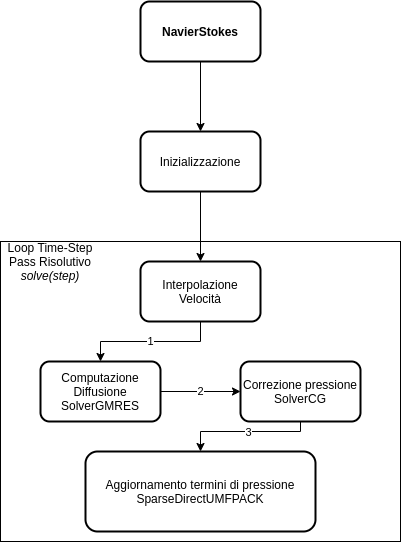
\includegraphics[width=\linewidth]{diagrammi/diagrammiNavier.png}
            \caption{diagramma di flusso NavierStokes.}
        \end{figure}
        Una volta creato l'oggetto tramite:
        \begin{verbatim}
NavierStokes navierstokes(settings, triangulation);
        \end{verbatim}
        lo inizializziamo cosi:
        \begin{verbatim}
navierstokes.setup_system();
        \end{verbatim}

        \subsection{Passo risolutivo}
        Dopo aver inizializzato correttamente il modulo è possibile richiamare la funzione:
        \texttt{solve(int step)}
        per risolvere un singolo time-step della simulazione. Vediamo in dettaglio come avviene la risoluzione del time-step e cosa comporta.

        Il primo passo consiste nell'interpolare (\ref*{interpolazione}) le velocità, successivamente si effettuano i calcoli per la diffusione.
        L'interpolazione della velocità avviene per mezzo di oggetti \textbf{Function<dim>} messi a disposizione da dealii che ci permettono di computare in un dato punto una serie di valori in base a
        formule matematiche che impostiamo. Nel caso, per esempio, dell'immissione, all'interno dell'ugello, del flusso è stata create una funzione denominata \textbf{InletVelocity}; che in base alla coordinata
        del punto in cui si calcola la velocità e una serie di impostazioni iniziali, computa il corretto valore che il flusso assume in termini di velocità.
        In una mesh possono agire tante funzioni interpolative quante ce ne sono bisogno. Una volta interpolati tutti i valori di velocità si passa a calcolare l'effettiva diffusione del flusso.
        Per procedere al calcolo diffusivo bisogna innanzitutto assemblare il sistema e applicare e interpolare le condizioni al contorno.
        Una volta calcolati i valori al contorno vengono applicati al sistema, che attraverso un solver GMRES (offerto sempre da dealii) computa la diffusione.

        Dopo aver calcolato la diffusione del fluido bisogna proiettare e correggere per il termine di pressione. Per computare l'apporto dato dalla pressione al fluido
        ci avvaliamo di un Solver CG (\texttt{Conjugate Gradient}, o gradiente coniugato) che implementa metodi per la risoluzione di sistemi lineari di matrici reali simmetriche positive.

        Ultimata la proiezione passiamo ad aggiornare le strutture dati che descrivono i valori di pressione utilizzando \textbf{SparseDirectUMFPACK}: un solver di sistemi lineari non simmetrici.
        Concluso quest'ultimo passaggio il programma ha correttamente simulato il movimento del flusso all'interno della mesh utilizzando le equazioni di Navier-Stokes (\ref*{navierstokes}).
        \subsection{Sistemi non lineari}
        Il modulo Navier Stokes è stato impelementato anche in una versione capace di risolvere sistemi di equazioni non lineari.
        Affinché il modulo riesca in questo intento è stato necessario introdurre uno schema risolutivo di tipo Newton-Raphson (\ref*{newtonraphson}).
        Per utilizzare questa versione è necessario introdurre due ulteriori impostazioni ricavate sempre dall'oggetto \texttt{Settings}: il numero di iterazioni 
        ammesse e la tolleranza per il metodo Newton-Raphson. 
        Avendo inizializzato correttamente il modulo nella sua versione non lineare, si passa alla risoluzione dei time-step. Per ogni step viene assemblato il problema non lineare, si controllano eventuali
        errori residui e si passa al controllo della convergenza della soluzione. Una volta che abbiamo appurato errori e convergenza si assembla la tangente del sistema e si impongono le condizioni di Dirichlet.
        A questo punto abbiamo convertito un sistema non lineare in un sistema linearizzato che possiamo risolvere tradizionalmente. 
    \section{Temperatura e Laser}\label{5:temperaturelaser}
    Analizziamo ora i componenti che sono responsabili per la simulazione del trasferimento di calore all'interno del simulatore, fondamentali per studiare il comportamento del flusso di
    particelle e il comportamento dello stesso nell'intorno della superficie su cui depositare il materiale.
    \begin{figure}[H]
        \centering
        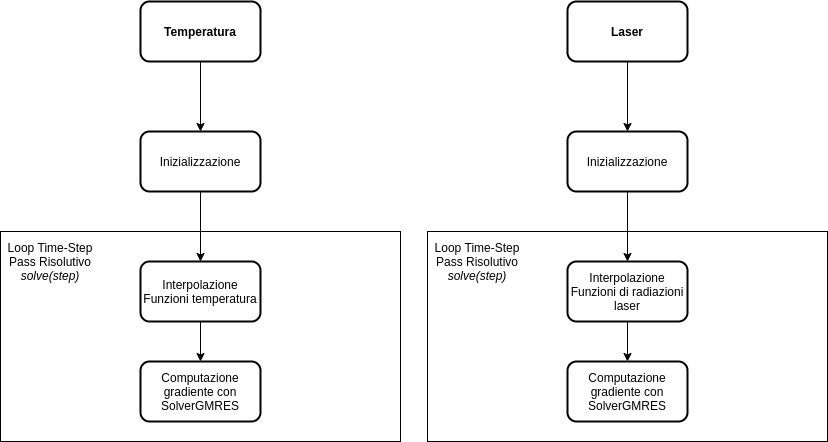
\includegraphics[width=\linewidth]{diagrammi/diagrammiTemp.png}
        \caption{diagramma di flusso Temperatura e laser.}
    \end{figure}
    L'inizializzazione dei moduli è simile a quella che abbiamo già effettuato per \ref{5:navierstokes}:
    \begin{verbatim}
Temperature temperature(settings,triangulation);
temperature.setup_system();
    \end{verbatim}

    \begin{verbatim}
Laser laser(settings,triangulation);
laser.setup_system();
    \end{verbatim}
    di seguito analizziamo nel dettaglio le differenze fra i due moduli.

    \subsection{Temperatura}\label{5:temperatura}
    L'inizializzazione del modulo temperatura comporta la valorizzazione, attraverso l'oggetto \textbf{Settings}, di diverse variabili necessarie a regolare il comportamento del modulo.
    Riportiamo di seguito alcune variabili particolarmente rilevanti:

    \begin{itemize}
        \item Tempo di applicazione dell'effetto \texttt{Plateu}
        \item Temperatura massima e minima
        \item Temperatura in prossimità dell'ingresso dell'ugello
    \end{itemize}

    Successivamente alla valorizzazione delle variabili, vengono inizializzate le strutture dati relative ai gradi di libertà del modulo temperatura, e i relativi vincoli.
    Il modulo temperatura prevede una correzione in fase di risoluzione del time-step che necessita di strutture sincronizzate con time-step precedenti, questo implica la creazione e la gestione di
    vettori contenenti informazioni "in ritardo" rispetto alla simulazione di uno e due time-step.
    Il passo finale dell'inizializzazione riguarda la prima interpolazione delle strutture contenenti i gradi di libertà con le rispettive condizioni iniziali.
    Risulta molto simile anche il resto del funzionamento del modulo temperatura rispetto a \ref*{5:navierstokes}, infatti una volta inizializzato il componente si passa
    alla computazione dello step corrente, sempre attraverso una funzione \texttt{solve(step)}. Il solver utilizzato in questo modulo rimane \textbf{SolverGMRES} come in \ref*{5:navierstokes}.
    La differenza con il modulo precedente sta ovviamente nel tipo di condizioni al contorno e nel tipo di funzioni che vengono computate per ogni punto.
    Vengono infatti interpolati i valori di temperatura del flusso e non più di velocità, per ogni cella della mesh. Per esempio nel caso dell'ogetto preso in esame si computa una zona di alta temperatura presso
    la parte iniziale del condotto dell'ugello, che nel corso della simulazione influenza il flusso passante per esso.
    Il modulo temperatura è intrinsicamente collegato a quello del laser \ref*{5:laser} e entrambi, congiuntamente a \ref*{5:navierstokes}, influenzano le proprietà delle particelle (\ref*{5:particelle}).

    \subsection{Laser}\label{5:laser}
    Questo modulo si occupa di simulare l'effetto di un fascio laser all'interno dell'ugello, che scalda il flusso e le particelle che lo attraversano influenzandone il comportamento.
    L'inizializzazione del modulo è simile a quella che abbiamo già effettuato per \ref{5:navierstokes} e \ref*{5:temperatura}, in questo caso, però, necessitiamo di solo due proprietà da \textbf{Settings}:
    \begin{itemize}
        \item La potenza del fascio laser
        \item Il raggio del fascio laser
    \end{itemize}
    inoltre sono presenti meno strutture dati. In particolare non avendo bisogno di risultati antecedenti al passo risolutivo corrente non ci sono strutture che referenziano stati precedenti come nel modulo temperatura.
    Prima di terminare l'inizializzazione, come di consueto ormai, interpoliamo le \textbf{Function<dim>} specifiche per il modulo laser con la struttura che gestisce i gradi di libertà (\textbf{DoFHandler}).
    Successivamente in fase di computazione del time-step ci avvaliamo un'altra volta di un \textbf{SolverGMRES} come in \ref{5:navierstokes} e \ref*{5:temperatura}.


    \section{Particelle}\label{5:particelle}
    Il modulo che gestisce le particelle è stato realizzato sulla base di una struttura offerta dalla libreria dealii \ref*{dealii}, \textbf{Particle<dim,spacedim>} che analizzeremo di seguito.
    La classe Particle rappresenta una particella singola all'interno di un dominio caratterizzato da un oggetto \textbf{Triangulation<dim,spacedim>}. Particle agisce come
    struttura dati per una singola particella al cui interno troviamo diverse informazioni fondamentali per la corretta simulazione della stessa, tra queste informazioni riportiamo di seguito le
    più utilizzate all'interno del progetto:
    \begin{itemize}
        \item Indice della particella (un identificativo univoco all'interno della simulazione)
        \item Posizione della particella nel sistema di riferimento della dominio intero
        \item Posizione della particella nel sistema di riferimento della cella in cui risiede
        \item Un vettore di proprietà personalizzabili in base alle necessità della simulazione. In questo progetto il vettore viene utilizzato per salvare informazioni quali velocità e temperatura della particella.
    \end{itemize}
    Analogamente a quanto utilizzato per gestire i gradi di libertà di \ref*{5:navierstokes}, \ref*{5:temperatura} e \ref*{5:laser}, dealii offre un oggetto in grado di manipolare in maniera controllata e precisa
    le particelle di una simulazione: \textbf{ParticleHandler<dim,spacedim>}. La classe ParticleHandler infatti espone diversi accessori per iterare particelle in un particolare dominio.
    \begin{figure}[H]
        \centering
        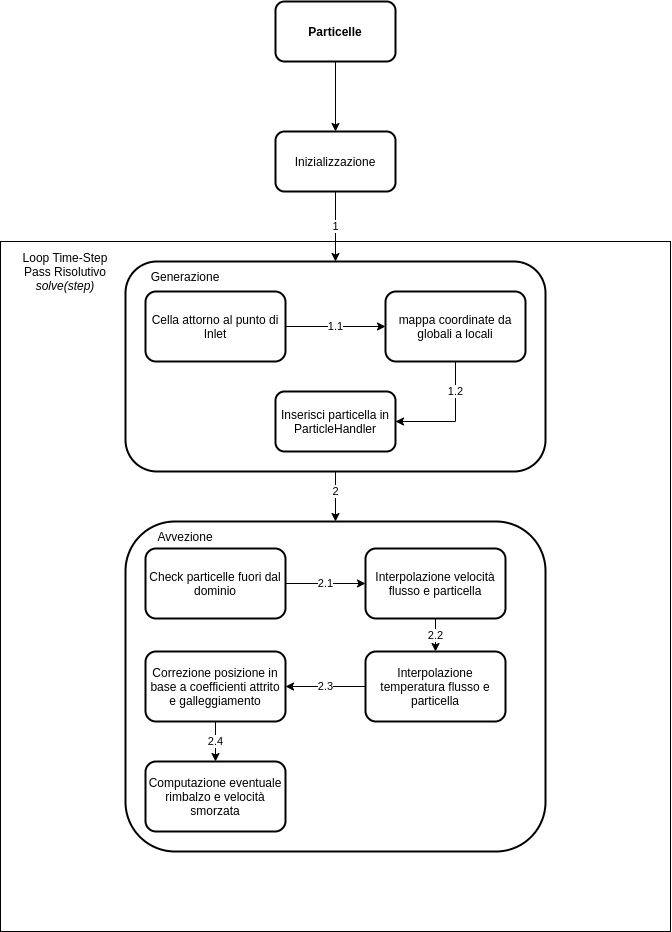
\includegraphics[width=\linewidth]{diagrammi/diagrammiParticelle.png}
        \caption{diagramma di flusso Temperatura e laser.}
    \end{figure}
    
    Ovviamente anche in questo modulo vi è una fase di inizializzazione eseguita però diversamente dagli altri:
    \begin{verbatim}
ParticlesDynamic particles_dynamic(settings,
                                   navierstokes,
                                   temperature,
                                   laser,
                                   triangulation);

    particles_dynamic.generate_particles();
    \end{verbatim}
    Infatti notiamo che quando creiamo l'oggetto principale del modulo, \textbf{ParticlesDynamic}, passiamo un riferimento agli altri moduli creati in precedenza. Questo perché, come anticipato,
    le particelle sono fortemente influenzate dai risultati dei moduli precedenti.
    Le impostazioni (\ref*{settings}) che vengono passate a questo modulo riguardano i principali aspetti che si vogliono parametrizzare all'interno di una simulazione di particelle,
    per la singola particella. Di seguito è riportata una lista delle più importanti:
    \begin{itemize}
        \item Massa della particella
        \item Durata della generazione delle particelle come flusso in entrata (per quanto tempo generiamo particelle)
        \item Densità della particella
        \item Diametro della particella
        \item Temperatura iniziale delle particelle
        \item Calore specifico
        \item Rateo di assorbimento calore
        \item Coefficiente di convezione
    \end{itemize}
    Inoltre al posto della funzione \texttt{setup\_system()} troviamo \texttt{generate\_particles()} che, come si evince
    dal nome scelto, è responsabile della generazione delle particelle all'interno della simulazione.
    Analizziamo ora le due principali funzionalità che offre il modulo di particelle: la generazione e l'avvezione delle stesse.
        \subsection{Generazione}
        Per rendere facilmente personalizzabile il processo di generazione particelle è stato realizzato un sottomodulo capace di interpretare determinate celle marcate
        come sorgenti di particelle. Questo permette di utilizzare diverse mesh e diverse sorgenti senza il bisogno di dover modificare il programma. Nel caso preso
        in esame, la generazione avviene in prossimità dell'ugello secondo i parametri passati in fase di inizializzazione.
        \begin{verbatim}
auto ref_cell = GridTools::find_active_cell_around_point(
                                dof_handler_temperature,
                                location);

Point<dim> ref_p = StaticMappingQ1<dim>::mapping
        .transform_real_to_unit_cell(ref_cell, location);

auto it =  particle_handler.insert_particle(Particles::Particle<dim>(
                                                location,
                                                ref_p,
                                                next_particle_index),
                                            ref_cell);
        \end{verbatim}
        Notiamo come dopo aver calcolato, secondo i criteri selezionati, il punto dove collocare la particella (\texttt{location}),
        dobbiamo effettuare alcune trasformazioni prima di crearla. In particolare occorre prima di tutto trovare la cella attorno al punto scelto attraverso l'accessore \textbf{GridTools},
        mappare le coordinate sul sistema di riferimento della cella trovata e infine inserire attraverso il ParticleHandler la particella. In questa fase nella particella inizalizziamo anche
        il vettore di proprietà con la temperatura iniziale ricavata attraverso le impostazioni.
        \subsection{Avvezione}
        L'avvezione delle particelle avviene nello stesso ciclo discretizzato degli altri moduli, dopo aver completato tutti i relativi calcoli dell'iterazione corrente.
        Il procedimento iniziale per procedere al calcolo del movimento delle particelle consiste in un iterazione attraverso tutte le particelle contenute nel \textbf{ParticleHandler}:
        \begin{verbatim}
for (auto p = particle_handler.begin();
        p != particle_handler.end();
        p++)
        \end{verbatim}
        all'interno di questo ciclo, in ordine, controlliamo se alcune particelle sono uscite dai confini del dominio in un iterazione precedente e le eliminiamo.
        Questo controllo è possibile sempre grazie a \texttt{find\_active\_cell\_around\_point()} che genera un eccezione in caso la particella non sia all'interno di una cella.
        Successivamente, per ogni modulo precedentemente descritto, ricaviamo dalla cella in cui si trova la particella informazioni riguardanti velocità del flusso, temperatura del flusso e
        potenza del fascio laser. Dopo aver correttamente recuperato queste informazioni possiamo aggiornare le proprietà della particella e procedere al calcolo della nuova posizione della stessa.
        Il calcolo della nuova posizione inizia con il recupero della velocità della particella allo step precedente, attraverso le proprietà precedentemente citate. Una volta recuperato lo stato precedente
        iniziamo l'interpolazione tra la velocità precedente della particella e la velocità del flusso nella cella dove risiede la particella. Ogni interpolazione avviene per ogni componente
        (\begin{math}
        x,y,z
        \end{math} nel nostro caso).
        Una volta terminata l'interpolazione con la velocità del flusso consideriamo il coefficiente d'attrito dinamico e il fattore di galleggiamento:
        \begin{verbatim}
auto drag_force = 0.5
                  * drag_coefficient
                  * fluid_density
                  * particle_area
                  * relative_velocity;

auto buoyancy = vector_gravity * particle_density
                * particle_volume
                *((particle_density - fluid_density)
                / particle_density);
        \end{verbatim}
        che inevitabilmente influenzeranno la velocità calcolata appena prima. Successivamente si introducono i calcoli per aggiornare la temperatura della particella,
        in particolare si considera sia il fascio laser che la temperatura del fluido. In termini pratici calcoliamo quanto calore viene assorbito dalla singola particella
        da entrambi i fattori:
        \begin{verbatim}
auto laser_power_absorption =  0.25 
                            * particle_absorptivity_rate 
                            * laser_field;
auto particle_fluid_convection = particle_convection_coefficient *
                (p->get_properties()[num_temperature]
                - temperature_interpolated_field)
                *particle_area;
auto new_particle_temperature =
        p->get_properties()[num_temperature]
            + ((dt / (particle_mass * particle_specific_heat)) *
            (laser_power_absorption - particle_fluid_convection));
        \end{verbatim}
        Terminate queste computazioni abbiamo valori aggiornati per temperatura e velocità e possiamo procedere al calcolo della uova posizione della particella.
        Banalmente possiamo calcolare la nuova posizione aggiungendo a quella corrente la nuova velocità moltiplicata per il delta temporale che intercorre fra due time-step:

        \begin{verbatim}
Point<dim> new_location = current_location + dt * new_particle_velocity;
        \end{verbatim}
        Prima di confermare la posizione e assegnarla alla particella, però, dobbiamo controllare la presenza di eventuali rimbalzi o collisioni.
        Per fare ciò controlliamo se la nuova location risiede sempre all'interno della mesh, se così non fosse allora dobbiamo procedere a calcolare il rimbalzo della particella.
        La collisione, e il relativo rimbalzo, viene calcolato iterando tutti i lati della mesh considerati come "muri" (superfici che non possono essere attraversate, opportunamente marcate)
        e controllando, per ognuno di essi, se la particella si trova in prossimità di una delle facce del muro. In caso di esito positivo si procede a calcolare se il segmento descritto dalle posizioni
        (vecchia e nuova) interseca la superficie, o faccia, del muro. Se il segmento effettivamente interseca la superficie si procede con il calcolo del vettore di rimbalzo e, quindi, la corretta posizione
        della particella.
        Il rimbalzo oltre ad influenzare la direzione è responsabile anche di una diminuzione di velocità della particella, regolata dalle leggi degli urti.
        Dopo aver calcolato anche l'eventuale rimbalzo possiamo finalmente assegnare alla particella la nuova posizione e i nuovi valori di temperatura e velocità.
        Questi calcoli, come già accennato, vengono ripetuti per ogni particella, per ogni step di simulazione; appare evidente quindi che al crescere del numero delle particelle e dei gradi di libertà degli altri moduli,
        la simulazione diventa sempre più onerosa in termini di risorse computazionali.

    \section{Parallelizzazione}\label{parallelizzazione}
    I moduli \ref*{5:navierstokes} e \ref*{5:temperaturelaser} utilizzano gli oggetti del namespace dealii \texttt{WorkStream} \cite{TKB16} per operare su più thread (o più processori). 
    WorkStream si basa interamente su \ref*{tbb} per bilanciare il carico di lavoro tra thread e su MPI per parallelizzare il lavoro su più calcolatori, condividendo informazioni e memoria.
    WorkStream rende disponibile a ogni calcolatore una copia dei DoFHandler in locale, mentre per matrici globali e vettori di soluzione condivide solo una parte (relativa ai propri calcoli).
    Una volta che il calcolatore ha a disposizione tutto il necessario esegue le computazioni necessarie e restituisce il risultato. Se un thread finisce una computazione con largo anticipo allora gli algoritmi di bilanciamento 
    di TBB reindirizzeranno il carico di task sul thread scarico. 
    Di seguito, un esempio di parallelizzazione utilizzando WorkStream:
    \begin{verbatim}
WorkStream::run(
    IteratorPair(IteratorTuple(ns.dof_handler_velocity.begin_active(),
                            dof_handler_temperature.begin_active())),
    IteratorPair(IteratorTuple(ns.dof_handler_velocity.end(),
                            dof_handler_temperature.end())),
        cell_worker_active,
        copier_active,
        T_ScratchData(*this, ns),
        T_CopyData(*this));
    \end{verbatim}
    \begin{figure}[H]
        \centering
        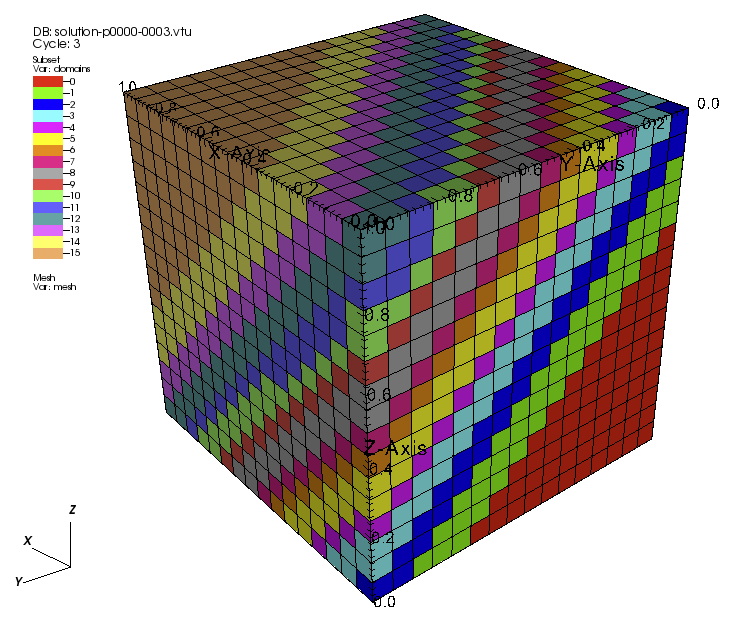
\includegraphics[width=\linewidth]{figure/distributedmesh.png}
        \caption{Esempio di mesh distribuita su più thread, differenziati per colore.}
    \end{figure}
    Con dealii è possibile anche distribuire gli oggetti Triangulation, entreremo nel dettaglio di questo particolare nella sezione Conclusioni e sviluppi futuri (\ref*{DistribuzioneTriangulation}).
    
    \section{Output}\label{5:output}
    Dopo aver effettuato i calcoli di tutti i moduli è necessario, per ogni step, esportare i dati computati per renderli fruibili in programmi di postprocessing e visualizzazione (\ref*{visualizzazione}).
    Per rendere il processo di output il più omogeneo possibile, ogni modulo implementa una funziona di output chiamata \texttt{output\_results()} che gestisce in maniera autonoma la creazione dei file di output
    secondo i formati scelti per ogni modulo.
    Tutti i moduli tranne quello di simulazione particelle utilizzano un oggetto condiviso per generare un file con estensione \texttt{VTK}, facilmente importabile in \textbf{Paraview}(\ref*{paraview}).
    L'oggetto utilizzato, ancora una volta offerto da dealii (\ref*{dealii}), è \textbf{DataOut<dim>} che permette di esportare le strutture \textbf{DoFHandler} utilizzate durante le simulazioni.
    DataOut offre una funzione denominata \texttt{build\_patches()} che itera su tutte le celle di una mesh (o Triangulation) salvate all'interno di un DoFHandler, precedentemente aggiunto all'oggetto
    DataOut, salvando tutte le informazioni di output in memoria. Una volta che sono state generate le informazioni di output è possibile invocare la funzione \texttt{write()} di DataOut, indicando un formato,
    per salvare su file ciò che è stato generato con \texttt{build\_patches()}. Questo approccio rende possibile salvare in più formati gli stessi dati in maniera facile e veloce.

    \paragraph{Navier-Stokes}
    All'interno del modulo Navier-Stokes la funzione di output aggiunge i seguenti DoFHandler all'oggetto DataOut:
    \begin{verbatim}
data_out.add_data_vector(dof_handler_velocity,
                    u_n,
                    "velocity",
                    stokes_component_interpretation);
data_out.add_data_vector(dof_handler_pressure, pres_n, "pressure");
    \end{verbatim}
    Si evince dal listato che il modulo Navier-Stokes fornisce in output informazioni riguardo la velocità e la pressione del fluido.
    Una volta passati entrambi gli oggetti a DataOut possiamo richiamare \texttt{build\_patches()} e passare al prossimo modulo.

    \paragraph{Temperatura}
    Analogamente a quanto fatto per il modulo precedente, e con le stesse istruzioni, aggiungiamo a DataOut il DoFHandler del modulo temperatura e costruiamo i dati di output.

    \paragraph{Laser}
    Identicamente al modulo temperatura, alleghiamo a DataOut le strutture riguardanti il fascio laser all'interno dell'ugello.

    \paragraph{Particelle}
    Essendo la struttura dei dati delle particelle completamente differente da quella degli altri moduli, anche il processo di output è sostanzialmente diverso.
    Il formato del file prodotto dal modulo particelle è un \texttt{CSV (comma separated values)}, poiché si tratta di generare una lista di particelle e valori associati.
    Per ogni step viene generato un file CSV denominato in base al numero di step corrente (al fine di poter importare gruppi di file in Paraview) al cui interno disponiamo
    i dati delle particelle, in modo tale che ogni particella occupi una riga del file. In una singola riga del file troviamo tutte le informazioni necessarie all'analisi
    della simulazione delle particelle:
    \begin{itemize}
        \item Posizione (divisa per componenti x, y, z)
        \item Temperatura
        \item Temperatura Fluido
        \item Velocità (divisa per componenti x, y, z)
        \item Velocità fluido (divisa per componenti x, y, z)
        \item Potenza Laser
        \item Identificatore Particella
    \end{itemize}

    Tutti i file prodotti, due per ogni step considerando che le particelle scrivono su un file separato dal resto dei moduli, vengono salvati all'interno di una cartella
    di output precedentemente specificata nel file di parametri (\ref*{input}). I file vengono denominati in modo tale che poi possano essere importati in Paraview
    in gruppi, ovvero seguendo questo pattern \texttt{nomeFile\_numeroStep.estensioneFile}, per esempio per i moduli che esportano VTK abbiamo \texttt{output\_0001.vtk}.
